\section{Approfondimenti su alcuni bilanci}

In questa sezione vengono analizzate alcune equazioni di bilancio
 in forma differenziale (è quindi necessario che queste equazioni siano
 valide!):
 vengono usate sia la rappresentazione euleriana sia la rappresentazione
 lagrangiana, al fine di ottenere la migliore comprensione dei fenomeni 
 fisici coinvolti.
 
Si indicano con $\bm{x}_0$ le coordinate lagrangiane, solidali con il 
 continuo; si indicano con $\bm{x}$ le coordinate euleriane.
I due sistemi di coordinate sono legati tra di loro dalle relazioni
\begin{equation}
\begin{aligned}
 \bm{x} = \bm{x}(\bm{x}_0,t) \\
 \frac{D \bm{x}}{D t} = \left.\frac{\partial \bm{x}}{\partial t}\right|_{\bm{x}_0} = 
 \bm{u}
\end{aligned}
\end{equation}
La derivata $\partial/\partial t$ indica la derivata temporale fatta
 a coordinata euleriana $\bm{x}$ costante. La derivata materiale 
 $D/D t$ indica la derivata fatta "a coordinata lagrangiana" costante
 e rappresenta quindi la variazione temporale di una quantità legata
 alla particella materiale, che si muove come il continuo, per la definizione
 di coordinate materiali.

\noindent
Il legame tra $D/Dt$ e $\partial/\partial t$ si trova utilizzando le
 regole di derivazione per funzioni composte. Scrivendo la funzione generica $f$ come
\begin{equation}
 f(\bm{x},t) = f(\bm{x}(\bm{x}_0,t),t)
  = f_0(\bm{x}_0,t) = f_0(\bm{x}_0(\bm{x},t),t) ,
\end{equation}
%
si ottiene
\begin{equation}
 \frac{D}{Dt} f = \left.\frac{\partial}{\partial t}\right|_{\bm{x}_0} f(\bm{x},t) =
   \left.\frac{\partial}{\partial t}\right|_{\bm{x}_0} f(\bm{x}(\bm{x_0},t),t) = 
   \left.\frac{\partial f}{\partial t}\right|_{\bm{x}} +
   \left.\frac{\partial \bm{x}}{\partial t}\right|_{\bm{x}_0} \cdot
   \left.\frac{\partial f}{\partial \bm{x}}\right|_{t}
   = \frac{\partial f}{\partial t} +
    \bm{u} \cdot \bm{\nabla} f .
\end{equation}

%\noindent
%Questo operatore può quindi essere interpretato come trasporto della 
% quantità $f$ dovuto a un campo $\bm{u}$.

%\noindent
%Può essere utile 



\subsection{Continuità}
%
L'equazione di continuità può essere riscritta mettendo in evidenza la derivata materiale
\begin{equation}
 \frac{\partial \rho}{\partial t} + \bm{\nabla} \cdot (\rho \bm{u}) = 0 
  \quad  \rightarrow  \quad 
  \frac{D\rho}{Dt} = -\rho \bm{\nabla} \cdot \bm{u}
\end{equation}
%
\'E possibile dimostrare\footnote{I più curiosi, cerchino ``fornmula di Jacobi''.} la relazione $DJ/Dt = J \bm{\nabla} \cdot \bm{u}$, dove
 $J$ indica il determinante del gradiente $\partial \bm{x}/\partial 
 \bm{x}_0$, si può scrivere l'equazione in coordinate lagrangiane,
 dopo averla moltiplicata per $J$ ($\ne 0$)
\begin{equation}
 J \frac{D\rho}{Dt} = - \rho \frac{DJ}{Dt} \Rightarrow
 \frac{D (J\rho)}{Dt} = 0 \Rightarrow J \rho = \rho_0
\end{equation}
%
La variazione della densità di una particella
 materiale è legata alla variazione del volume della stessa (ricordare
 che $dv = J dV$). Questa conclusione è ragionevole se si pensa che
 la massa della particella materiale si conserva ($dm = \rho dv = 
 \rho_0 dV$).
%
\begin{remark}
Il vincolo di incomprimibilità rappresenta la costanza del volume della 
 particella materiale. Il volume $dv$ coincide con il volume di riferimento $dV$, implicando $J \equiv 1$ e quindi  $\bm{\nabla} \cdot \bm{u} = 0$.
\end{remark}



\subsection{Quantità di moto}

L'equazione della quantità di moto è
\begin{equation}
 \rho \left\{ \frac{\partial \bm{u}}{\partial t} +
   \left( \bm{u} \cdot \bm{\nabla} \right) \bm{u} \right\} = 
   \bm{\nabla} \cdot \mathbb{T} + \bm{f}
\end{equation}
dove con $\mathbb{T}$ è stato indicato il tensore degli sforzi,
 che per un fluido newtoniano è $\mathbb{T} = -p \mathbb{I} + \mathbb{S}$
 con $\mathbb{S} = 2 \mu \mathbb{D} + \lambda \left( 
 \bm{\nabla} \cdot \bm{u} \right) \mathbb{I}$ e $\mathbb{D} = \frac{1}{2}
 \left[ \bm{\nabla}\bm{u} + \bm{\nabla}^T \bm{u} \right]$ il tensore
 velocità di deformazione, parte simmetrica del gradiente della velocità.
%
Introducendo la derivata materiale, si ritrova una forma ``familiare''
 del secondo principio della dinamica
\begin{equation}
 \rho\frac{D\bm{u}}{D t} = \bm{\nabla} \cdot \mathbb{T} + \bm{f}
  \qquad \Rightarrow \qquad
 \rho\bm{a} = \bm{\nabla} \cdot \mathbb{T} + \bm{f}
\end{equation}
%
\paragraph{Richiami di geometria delle curve nello spazio.}
Una curva è un luogo di punti che può essere parametrizzato tramite un
 parametro solo.
La parametrizzazione $\bm{r}(t)$ della curva $\bm{r}$ è definita regolare 
 se $d\bm{r}/dt \ne 0$. Si definisce poi una parametrizzazione regolare
 particolare, l'ascissa curvilinea $s$ tale per cui $\left| d\bm{r}(s)/ds
 \right| = 1, \forall s \in (a,b)$.

\noindent 
Nel seguito si introduce brevemente la \textbf{terna di Frenet} 
 $\left\{\bm{\hat{t}}, \bm{\hat{n}}, \bm{\hat{b}} \right\}$, formata
 dai versori tangente, normale e binormale, in funzione dell'ascissa
 curvilinea.
%
Si dimostra che
\begin{equation}
 \bm{\hat{t}}(s) = \dfrac{d\bm{r}}{ds}
\end{equation}
%
La derivata seconda della posizione $\bm{r}$, cioè la derivata prima del
 versore tangente $\bm{\hat{t}}$ è legata al versore normale
 $\bm{\hat{t}}$, tramite la curvatura $k = \left| \frac{d\bm{\hat{t}}}{
 ds} \right|$.
\begin{equation}
 \bm{\hat{n}} = \dfrac{\frac{d\bm{\hat{t}}}{ds}}
    {\left|\frac{d\bm{\hat{t}}}{ds} \right|} 
  \qquad \Rightarrow \qquad
 \dfrac{d\bm{\hat{t}}}{ds} = k \bm{\hat{n}}
\end{equation}
%
Il versore binormale è definito a completare la terna ortonormale 
 destrorsa
\begin{equation}
 \bm{\hat{b}} = \bm{\hat{t}} \times \bm{\hat{n}} 
\end{equation}
%
Per completezza e senza troppo sforzo si calcolano anche le derivate 
 di tali versori, ricordando che hanno modulo unitario e costante,
 e formano una terna ortogonale in ogni punto, introducendo la definizione
 della torsione $\tau = \frac{d \bm{\hat{n}}}{ds}\cdot \bm{b}$.
\begin{equation}
\begin{aligned}
& \qquad \qquad \qquad \qquad \qquad \qquad \qquad \qquad 
  \qquad \qquad \qquad \qquad \quad
 \frac{d \bm{\hat{t}}}{ds} = k \bm{\hat{n}} \\
& \begin{cases}
 \bm{\hat{n}}'\cdot \bm{\hat{n}} = 0 \\
 \bm{\hat{n}}'\cdot \bm{\hat{t}}+\bm{\hat{t}}'\cdot \bm{\hat{n}} = 0 \\
 \bm{\hat{n}}'\cdot \bm{\hat{b}} = \tau \\
 \end{cases} \Rightarrow \quad
 \begin{cases}
 \bm{\hat{n}}'\cdot \bm{\hat{n}} = 0   \\
 \bm{\hat{n}}'\cdot \bm{\hat{t}} = -k  \\
 \bm{\hat{n}}'\cdot \bm{\hat{b}} = \tau \\
 \end{cases} \qquad \quad \quad \Rightarrow \quad 
  \frac{d \bm{\hat{n}}}{ds} = - k \bm{\hat{t}} + \tau \bm{\hat{b}} \\
& \begin{cases}
 \bm{\hat{b}}'\cdot \bm{\hat{b}} = 0 \\
 \bm{\hat{b}}'\cdot \bm{\hat{t}} + \bm{\hat{t}}'\cdot \bm{\hat{b}} = 0 \\
 \bm{\hat{b}}'\cdot \bm{\hat{n}} + \bm{\hat{n}}'\cdot \bm{\hat{b}} = 0 \\
 \end{cases} \Rightarrow \quad
 \begin{cases}
 \bm{\hat{b}}'\cdot \bm{\hat{b}} = 0 \\
 \bm{\hat{b}}'\cdot \bm{\hat{t}} = -\bm{\hat{t}}'\cdot \bm{\hat{b}} = 0 \\
 \bm{\hat{b}}'\cdot \bm{\hat{n}} = -\bm{\hat{n}}'\cdot \bm{\hat{b}} = -k\\
 \end{cases} \Rightarrow \quad
  \frac{d \bm{\hat{b}}}{ds} = - \tau \bm{\hat{n}} \\
\end{aligned}
\end{equation}
%
Se la parametrizzazione regolare della curva non è l'ascissa curvilinea,
 si può ricavare
\begin{equation}
 \frac{d\bm{r}}{dt} = \frac{ds}{dt}\frac{d\bm{r}}{ds} = 
  v \bm{\hat{t}}
\end{equation}
dove si è introdotto il modulo $v$ di quella che sarà la velocità $\bm{v}$
 quando $\bm{r}$ e $t$ saranno spazio e tempo.
In maniera analoga
\begin{equation}
 \frac{d\bm{\hat{t}}}{dt} = \frac{ds}{dt}\frac{d\bm{\hat{t}}}{ds} = 
  v k \bm{\hat{n}}
\end{equation}
 %
Se $\bm{r}$ e $t$ sono spazio e tempo, la velocità e l'accelerazione di un
 punto che ha come legge oraria $\bm{r}(t)$ sono
\begin{equation}
 \begin{aligned}
  \bm{v} & = \frac{d\bm{r}}{dt} = \frac{ds}{dt}\frac{d\bm{r}}{ds} = 
    v \bm{\hat{t}} \\
  \bm{a} & = \frac{d\bm{v}}{dt} =
   \frac{dv}{dt} \bm{\hat{t}} + v \frac{d\bm{\hat{t}}}{dt} =
   \frac{dv}{dt} \bm{\hat{t}} + v^2 k \bm{\hat{n}}
 \end{aligned}
\end{equation}
%
\begin{minipage}{0.60\textwidth}
\paragraph{Ritorno al bilancio della quantità di moto.} Inserendo la
 forma dell'accelerazione nell'equazione della quantità di moto e 
 proiettando lungo i versori della terna di Frenet
\begin{equation}
 \begin{cases}
  \rho \frac{dv}{dt} =  \bm{\hat{t}} \cdot \left(
     \bm{\nabla} \cdot \mathbb{T} + \bm{f} \right) \\
  \rho v^2 k = \bm{\hat{n}} \cdot \left(
     \bm{\nabla} \cdot \mathbb{T} + \bm{f} \right) \\
  0 = \bm{\hat{b}} \cdot \left(
     \bm{\nabla} \cdot \mathbb{T} + \bm{f} \right) \\
 \end{cases}
\end{equation}
L'analisi per componenti locali dell'equazione della quantità di moto permette di riconoscere che:
\end{minipage}
\hfill
\begin{minipage}{0.40\textwidth}
\begin{center}
   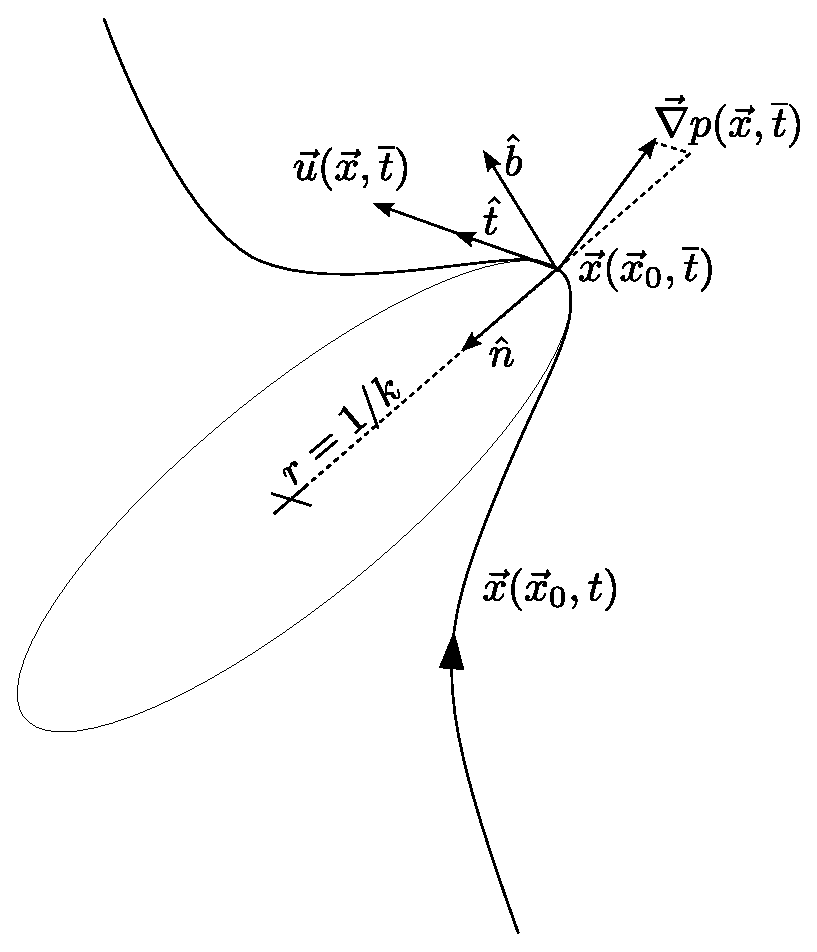
\includegraphics[width=1.0\textwidth]{./fig/frenet.eps}
\end{center}
\end{minipage}
\begin{itemize}
 \item la proiezione del termine forzante lungo la tangente alla traiettoria è la responsabile dell'accelerazione tangenziale della particella materiale;
 \item la proiezione del termine forzante lungo la normale alla traiettoria è la responsabile dell'accelerazione centripeta della particella maetriale e, di conseguenza, della curvatura della traiettoria;
 \item la proiezione della forzante lungo la direzione binormale è nulla.
\end{itemize}

\noindent
In assenza di forze di volume ($\bm{f}=0$) e sforzi viscosi
($\mathbb{T}=\mathbb{S}-p\mathbb{I}=-p\mathbb{I}$):
\begin{equation}
 \begin{cases}
  \rho \frac{dv}{dt} = - \bm{\hat{t}} \cdot \bm{\nabla} p \\
  \rho v^2 k         = - \bm{\hat{n}} \cdot \bm{\nabla} p \\
  0                  = - \bm{\hat{b}} \cdot \bm{\nabla} p \\
 \end{cases}
\end{equation}
%
e quindi:
\begin{itemize}
 \item l'accelerazione tangenziale è proporzionale alla proiezione del gradiente di pressione in direzione tangente alla tratiettoria;
 \item l'accelerazione centripeta, $v^2/r = v^2 k$, è proporzionale alla proiezione del gradiente di pressione in direzione normale alla tratiettoria. Il termine $\rho v^2 k$ è sempre positivo poichè prodotto di quantità positive: la curvatura di una linea è non negativa per come è definita, la densità è positiva, il modulo di un vettore è anch'esso non negativo. Il prodotto scalare tra la normale e il gradiente della pressione (derivata direzionale della pressione in direzione $\bm{\hat{n}}$) deve quindi essere negativo. La pressione quindi diminuisce, andando verso il centro del cerchio osculatore. Sempre dalla seconda equazione è immediato notare che la curvatura della traiettoria è proporzionale alla componente del gradiente di pressione lungo il versore normale;
 \item la proiezione del gradiente di pressione in direzione binormale a una traiettoria è nullo.
\end{itemize}
% Un'analisi della componente normale permette di ricavare, \textbf{sotto le
%  ipotesi fatte}, il legame tra la curvatura delle traiettorie delle
%  particelle fluide e il gradiente del campo di pressione.
% Il termine a sinistra dell'uguale è positivo
% La componente tangente fa aumentare 
%  il modulo della velocità, mentre la componente binormale deve essere nulla.
%Essendo il versore $\bm{\hat{n}}$ diretto verso il centro del cerchio
% osculatore (in parole povere è diretta verso l'interno della curva),
% la curvatura $k$ positiva, segue che la pressione deve diminuire lungo 
% $\bm{\hat{n}}$, cioè aumenta all'allontanarsi dal cerchio del centro
% osculatore (in parole altrettanto povere, ``verso l'esterno'').
%\textit{(Nemmeno a dirlo, la densità $\rho$ è positiva e il quadrato
%  del modulo della velocità $v^2$ è positivo.)}
%\noindent
%Dalla componente lungo $\bm{\hat{n}}$ si nota che il legame tra 
% la componente del gradiente della pressione in quella direzione è
% \textbf{proporzionale} alla curvatura della traiettoria della particella
% fluida.



\subsection{Vorticità}

L'equazione della vorticità in coordinate euleriane è
\begin{equation}
 \frac{\partial \bm{\omega}}{\partial t}
   + (\bm{u}\cdot\bm{\nabla}) \bm{\omega} =
 (\bm{\omega}\cdot\bm{\nabla}) \bm{u} + \nu \bm{\Delta} \bm{\omega}
\end{equation}

Se viene fatta l'ipotesi di viscosità nulla, il termine contenente il 
 laplaciano della vorticità non compare nell'equazione: questo termine
 è il responsabile della diffusione (isotropa per come è scritto) della
 vorticità.
 
L'equazione può essere quindi riscritta come:
 \begin{equation}
  \frac{D\bm{\omega}}{Dt} = (\bm{\omega} \cdot \bm{\nabla}) \bm{u}
 \end{equation}

\noindent 
Scritta in componenti
\begin{equation}
\begin{aligned}
  \frac{D \omega_i}{D t} = \omega_k \frac{\partial u_i}{\partial x_k} \\
\end{aligned}
\end{equation}

\noindent
Il termine di destra può essere riscritto come
\begin{equation}
\begin{aligned}
 \omega_k \frac{\partial u_i}{\partial x_k} & = 
 \omega_k \frac{\partial u_i}{\partial x_{0 l}}
      \frac{\partial x_{0 l}}{\partial x_k} = \qquad \qquad
      \left(u_i = \frac{D x_i}{D t}\right)  \\
 & = \omega_k \frac{D}{Dt} \left( \frac{\partial x_i}{\partial x_{0 l}}
    \right)\frac{\partial x_{0 l}}{\partial x_k} 
\end{aligned}
\end{equation}
Vale la relazione
\begin{equation}
 \frac{\partial x_i}{\partial x_{0 l}}
   \frac{\partial x_{0 l}}{\partial x_k} = \delta_{ik}
\end{equation}
Il termine di sinistra può essere riscritto come
\begin{equation}
 \frac{D \omega_i}{Dt} = \frac{D}{Dt} \left(\delta_{ik} \omega_k \right) =
 \frac{D}{Dt} \left( \frac{\partial x_i}{\partial x_{0 l}}
   \frac{\partial x_{0 l}}{\partial x_k} \omega_k \right)
\end{equation}

Inserendo nell'equazione della vorticità e sfruttando le proprietà
 della derivata del prodotto:
\begin{equation}
\begin{aligned}
 &  \frac{D}{Dt} \left(  \frac{\partial x_i}{\partial x_{0 l}}
   \frac{\partial x_{0 l}}{\partial x_k} \omega_k  \right)  - 
  \omega_k \frac{D}{Dt} \left( \frac{\partial x_i}{\partial x_{0 l}}
    \right)\frac{\partial x_{0 l}}{\partial x_k} = 0 \\
 &  \frac{\partial x_i}{\partial x_{0 l}} 
  \frac{D}{Dt} \left( \frac{\partial x_{0 l}}{\partial x_k} \omega_k
    \right) = 0
\end{aligned}
\end{equation}
Se la trasformazione non è singolare, risulta quindi
\begin{equation}
  \frac{D}{Dt} \left( \frac{\partial x_{0 l}}{\partial x_k} \omega_k
    \right) = 0  \quad \Rightarrow \quad
  \frac{\partial x_{0 l}}{\partial x_k} \omega_k = \omega_{l 0}
\end{equation}
e in conclusione, invertendo il gradiente della trasformazione delle
 coordinate
\begin{equation}\label{eqn:bilanci:vorticitàLagrange}
   \omega_k = \frac{\partial x_k}{\partial x_{0 l}}\omega_{l 0}
   \qquad , \qquad \bm{\omega} = \frac{\partial \bm{x}}{\partial \bm{x}_0}
      \bm{\omega}_0
\end{equation}

Si può quindi notare che la vorticità segue la stessa evoluzione
 di un segmento infinitesimo materiale, per il quale vale:
\begin{equation}
  d\bm{x} = \frac{\partial \bm{x}}{\partial \bm{x}_0}
      d\bm{x}_0
\end{equation}










 
